\chapter{Persona Vectors: Replication and Negative Result}
\label{ch:replication}

This chapter reports Experiments 1 and 2 in order. Experiment 1 replicates the published persona-vector extraction methodology on Gemma-2-9B-Instruct at 4-bit NF4 with the full Dubanowska control battery. Experiment 2 tests whether the validated direction transfers to inference-time drift detection in multi-turn dialogue on the same backbone and on Llama-3.1-8B-Instruct, in two extraction regimes. The chapter closes with the architectural cascade Experiment 2 induced: M2 dropped, M3 reverted to its v0.2 design, B3 deferred.

\section{Experiment 1: persona-vector replication on Gemma-2-9B at 4-bit}
\label{sec:experiment-1}

\subsection{Setup}

The backbone is Gemma-2-9B-Instruct\autocite{gemma2024} loaded in 4-bit NF4 with double quantisation and fp16 compute via bitsandbytes\autocite{bitsandbytes}, with eager attention (Gemma 2's softcap is broken on SDPA and Flash-Attention-2 in transformers releases at the project's pinned version)\autocite{transformers}. The hidden dimension is 3584 and the model has 42 transformer layers. The peak VRAM during contrast-prompt forward passes was 18.4 GB on the V100's 32 GB.

For each of three personas (cs\_tutor, historian, climate\_scientist), the contrastive-prompt generator produces 50 template-based contrast pairs covering the persona's worldview and self-fact topics. The split is hash-based on prompt id with $\texttt{test\_fraction} = 0.20$ and seed 42, producing 40 train pairs and 10 test pairs per persona, with the test set prompt-disjoint from the training set. Hidden states are pooled at the final prompt token (\texttt{pool=last}, \texttt{scope=prompt}) at four layers \{8, 12, 16, 20\}. The persona vector at each layer is the mass-mean difference of the train-split centroids. The probe is logistic regression on the 1-dimensional projection scores.

\subsection{Per-layer test AUROC}

Table~\ref{tab:experiment-1-auroc} reports the per-layer test \auroc{} for each persona. Train \auroc{} per persona ranges from 0.977 (cs\_tutor layer 8) to 1.000 across the higher layers; no signs of leakage. The global best layer (mean test \auroc{} argmax with per-persona-best tie-broken by lowest index) is layer 8 at mean \auroc{} 1.000. Figure~\ref{fig:auroc-heatmap} plots the same per-layer \auroc{} grid against the two Dubanowska control bands. The classifier band saturates near 1.0 across every (persona, layer) cell; the shuffled-label control sits at chance and the random-feature control sits well below the 0.70 weak floor.

\begin{figure}[H]
  \centering
  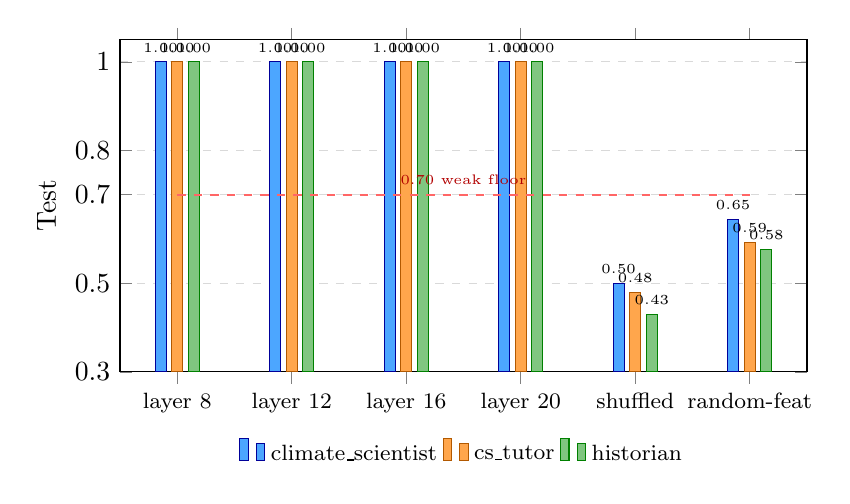
\begin{tikzpicture}
    \begin{axis}[
        width=0.85\textwidth,
        height=5.8cm,
        ybar,
        bar width=4pt,
        ymin=0.30, ymax=1.05,
        ytick={0.30, 0.50, 0.70, 0.80, 1.00},
        ylabel={Test \auroc{}},
        symbolic x coords={layer 8, layer 12, layer 16, layer 20, shuffled, random-feat},
        xtick=data,
        x tick label style={font=\footnotesize},
        enlarge x limits=0.1,
        legend style={at={(0.5,-0.18)}, anchor=north, legend columns=3, font=\footnotesize, draw=none},
        ymajorgrids=true,
        grid style={dashed, gray!30},
        nodes near coords style={font=\tiny, /pgf/number format/.cd, fixed, fixed zerofill, precision=2},
        nodes near coords,
      ]
      \addplot[fill=blue!50!cyan!70, draw=blue!60!black] coordinates {(layer 8, 1.00) (layer 12, 1.00) (layer 16, 1.00) (layer 20, 1.00) (shuffled, 0.50) (random-feat, 0.645)};
      \addplot[fill=orange!70, draw=orange!70!black]    coordinates {(layer 8, 1.00) (layer 12, 1.00) (layer 16, 1.00) (layer 20, 1.00) (shuffled, 0.48) (random-feat, 0.592)};
      \addplot[fill=green!55!black!50, draw=green!50!black] coordinates {(layer 8, 1.00) (layer 12, 1.00) (layer 16, 1.00) (layer 20, 1.00) (shuffled, 0.43) (random-feat, 0.576)};
      \legend{climate\_scientist, cs\_tutor, historian}
      \draw[dashed, red!60, thick] (axis cs:layer 8, 0.70) -- (axis cs:random-feat, 0.70) node[pos=0.5, above, font=\tiny, red!70!black] {0.70 weak floor};
    \end{axis}
  \end{tikzpicture}
  \caption{Experiment 1 per-layer test \auroc{} (\emph{layer 8}-\emph{layer 20} group) against Dubanowska defensive controls (\emph{shuffled} = shuffled-label, \emph{random-feat} = random-feature). The dashed line marks the 0.70 weak floor below which the random-feature control must sit for the main result not to be compromised. Source: \texttt{results/a11\_validation/20260425\_094657/}.}
  \label{fig:auroc-heatmap}
\end{figure}

\begin{table}[H]
  \centering
  \small
  \caption{Experiment 1 per-layer test \auroc{} for the persona-vector linear-separability probe. Held-out prompt-disjoint test split (10 pairs per persona, seed 42). Run \texttt{results/a11\_validation/20260425\_094657/}.}
  \label{tab:experiment-1-auroc}
  \begin{tabular}{lcccccc}
    \toprule
    \textbf{Persona} & \textbf{Layer 8} & \textbf{Layer 12} & \textbf{Layer 16} & \textbf{Layer 20} & \textbf{Best layer} & \textbf{Best \auroc{}} \\
    \midrule
    climate\_scientist & 1.000 & 1.000 & 1.000 & 1.000 & 8 & 1.000 \\
    cs\_tutor          & 1.000 & 1.000 & 1.000 & 1.000 & 8 & 1.000 \\
    historian          & 1.000 & 1.000 & 1.000 & 1.000 & 8 & 1.000 \\
    \bottomrule
  \end{tabular}
\end{table}

\subsection{Dubanowska defensive controls}

Two control conditions follow the Dubanowska protocol\autocite{dubanowska2025}. The shuffled-label control trains the probe on the same projections with permuted labels; the random-feature control trains the probe on prompt length rather than on the persona-vector projection. Both are averaged across $N = 10$ randomisations to dampen sampling noise.

\begin{table}[H]
  \centering
  \small
  \caption{Dubanowska defensive controls. Mean over $N = 10$ randomisations. The weak floor is 0.70; the random-feature control sits in the 0.58 to 0.65 band, the shuffled-label control at chance.}
  \label{tab:dubanowska}
  \begin{tabular}{lccc}
    \toprule
    \textbf{Persona} & \textbf{Shuffled-label range (4 layers)} & \textbf{Random-feature} & \textbf{Compromised?} \\
    \midrule
    climate\_scientist & 0.50 / 0.50 / 0.50 / 0.50 & 0.645 & No \\
    cs\_tutor          & 0.40 / 0.50 / 0.50 / 0.50 & 0.592 & No \\
    historian          & 0.40 / 0.50 / 0.40 / 0.40 & 0.576 & No \\
    \bottomrule
  \end{tabular}
\end{table}

The shuffled-label control sits at chance with the small dip below 0.5 explained by the variance on the $n = 10$ test set averaged over 10 randomisations. The random-feature control lands in the 0.58 to 0.65 band, well below the 0.70 weak floor. Per the Dubanowska protocol, the main signal is not compromised.

\subsection{Drift-signal sign convention}

A separate check confirms the drift-signal sign convention at the centroids. The function \texttt{DriftSignal.compute} returns $+1.000$ on the in-persona centroid and $-1.000$ (or $-0.99998$ for the historian, a float32 round-off) on the out-of-persona centroid for each persona at the global best layer. The $[-1, +1]$ mapping the mechanism specifications assume holds at the centroids exactly.

\subsection{UMAP visual sanity}

The UMAP projections of the per-layer hidden states, coloured by in-persona-versus-out-of-persona, separate cleanly for all three personas. Climate\_scientist and historian split along UMAP-2; cs\_tutor splits diagonally. The \auroc{} 1.000 is corroborated by the figures rather than being an artefact of dimension-reduction noise on the small test set. The UMAPs are committed to the run directory as \texttt{umap\_<persona>\_layer8.png}.

\subsection{Caveats}

Three caveats attach to the result. The \auroc{} 1.000 saturation across all four layers means the layer sweep does not discriminate, which is consistent with prompt-time activations being dominated by the explicit role instruction in the contrast prompt; this motivates Experiment 2's generation-scope re-extraction. The test set is small ($n = 10$ per persona), which makes the \auroc{} ceiling coarse: a single mis-ranked pair drops to 0.99. The Llama-3.1-8B replication of Experiment 1 was not run as a separate gate (Experiment 2 includes Llama in the generation-scope sweep, which serves as the cross-backbone check).

\subsection{Verdict}

Experiment 1's verdict is \textbf{confirmed}. The persona-vectors methodology replicates on Gemma-2-9B-Instruct at 4-bit NF4, on the (backbone, quantisation) cell that prior work had not tested, with the Dubanowska controls intact. The PRD's pre-registered proceed criterion ($\auroc{} \geq 0.80$ on held-out test) is met by a wide margin. Downstream mechanism specifications that depend on the persona-vector infrastructure proceed.

\section{Experiment 2: drift-trajectory sanity}
\label{sec:experiment-2}

The architectural question Experiment 1 does not answer is whether the validated direction transfers. Specifically: does the persona-vector projection, computed on a hidden state captured during multi-turn dialogue rather than on a contrast-prompt activation, move differentially between conversations where the model stays in persona and conversations where it drifts? M3's gate signal, M2's rerank scorer, and the broader v3 architectural commitment depend on the answer being yes. Experiment 2 tests it directly.

\subsection{Setup}

For each of the three personas, two synthetic six-turn conversations are hand-authored. The in-persona conversation has six turn-pairs with assistant turns that stay clearly in character. The drifting conversation has identical user turns (the experimental control) and assistant turns that drift progressively: in-persona at turns 1-2, subtle drift at turn 3 (a slight worldview contradiction or constraint violation), clearer drift at turns 4-5 (claims of expertise the persona does not have, opposite worldview stance), and a full break at turn 6 (refusing to stay in role).

This isolates the variable. The same prompt prefix, the same user turns, only the assistant generations differ. If the persona-vector projection tracks generation content, it should drop measurably between in-persona and drifting on the same turn pairs.

The sweep covers two backbones (Gemma-2-9B-Instruct, Llama-3.1-8B-Instruct), both at 4-bit NF4 + double quantisation, fp16 compute, eager attention. Two extraction regimes are tested: prompt-scope (\texttt{pool=last, scope=prompt}, the published recipe and the one Experiment 1 used) and generation-scope (\texttt{pool=mean, scope=generation}, the natural mitigation candidate suggested by Experiment 1's \auroc{} saturation across layers). Four layers per (backbone, scope) cell: \{8, 12, 16, 20\} on Gemma and \{6, 10, 14, 18\} on Llama, symmetric middle bands relative to each backbone's depth (Gemma 42, Llama 32). Three personas $\times$ 2 conditions $\times$ 6 turns gives 36 forward passes per cell.

The pre-registered proceed threshold is a mean drift delta $\mu_{\text{in}} - \mu_{\text{drift}} \geq +0.30$ in the correct direction (in-persona scoring more positive) for at least two of three personas. The kill criterion is a delta below $+0.10$ across all personas, in which case the persona-vector projection signal is judged not useful as a multi-turn drift gate and the M3 gate signal must be replaced.

\subsection{Per-cell summary}

Table~\ref{tab:experiment-2-summary} reports the per-(backbone, scope) summary. Per-layer verdicts (proceed, weak, refuted, inconclusive) are derived from the pre-registered rule and listed for each cell.

\begin{table}[H]
  \centering
  \small
  \caption{Experiment 2 per-cell summary. ``Best mean delta'' is over drift turns, signed so that in-persona scoring more positive is positive. ``Max $\lvert$delta$\rvert$'' is the largest absolute delta in any (persona, layer) sub-cell. The proceed threshold is $+0.30$.}
  \label{tab:experiment-2-summary}
  \begin{tabularx}{\textwidth}{l l l c r r X}
    \toprule
    \textbf{Backbone} & \textbf{Scope} & \textbf{Layers} & \textbf{Best layer} & \textbf{Best mean $\Delta$} & \textbf{Max $\lvert\Delta\rvert$} & \textbf{Per-layer verdicts} \\
    \midrule
    Gemma-2-9B 4-bit  & prompt     & 8, 12, 16, 20 & 12 & $-0.018$ & 0.101 (wrong direction) & inconclusive(8); refuted(12, 16, 20) \\
    Gemma-2-9B 4-bit  & generation & 8, 12, 16, 20 & 8  & $+0.004$ & 0.044                   & refuted(8, 12, 16, 20)               \\
    Llama-3.1-8B 4-bit & generation & 6, 10, 14, 18 & 14 & $+0.026$ & 0.103 (wrong direction) & refuted(6, 10, 14); inconclusive(18) \\
    \bottomrule
  \end{tabularx}
\end{table}

The proceed threshold is $+0.30$. The maximum absolute signal observed anywhere in the sweep is 0.103, in the wrong direction. The signal we would have needed to gate on is missing by an order of magnitude across every cell.

\begin{figure}[H]
  \centering
  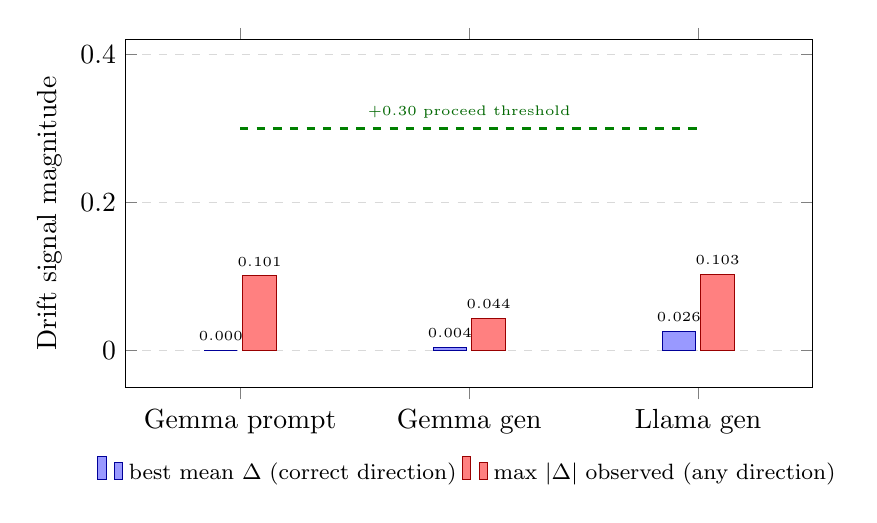
\begin{tikzpicture}
    \begin{axis}[
        width=0.85\textwidth,
        height=6.0cm,
        ybar,
        bar width=12pt,
        ymin=-0.05, ymax=0.42,
        ylabel={Drift signal magnitude},
        symbolic x coords={Gemma prompt, Gemma gen, Llama gen},
        xtick=data,
        enlarge x limits=0.25,
        legend style={at={(0.5,-0.18)}, anchor=north, legend columns=2, font=\footnotesize, draw=none},
        ymajorgrids=true,
        grid style={dashed, gray!30},
        nodes near coords style={font=\tiny, /pgf/number format/.cd, fixed, fixed zerofill, precision=3},
        nodes near coords,
      ]
      \addplot[fill=blue!40, draw=blue!60!black] coordinates {(Gemma prompt, 0.000) (Gemma gen, 0.004) (Llama gen, 0.026)};
      \addplot[fill=red!50, draw=red!60!black]   coordinates {(Gemma prompt, 0.101) (Gemma gen, 0.044) (Llama gen, 0.103)};
      \legend{best mean $\Delta$ (correct direction), max $|\Delta|$ observed (any direction)}
      \draw[dashed, green!50!black, thick] (axis cs:Gemma prompt, 0.30) -- (axis cs:Llama gen, 0.30) node[pos=0.5, above, font=\tiny, green!40!black] {$+0.30$ proceed threshold};
    \end{axis}
  \end{tikzpicture}
  \caption{Experiment 2 per-cell summary. Best mean $\Delta$ is the largest drift-delta in the correct direction (in-persona scoring more positive than drifting). Max $|\Delta|$ is the largest absolute delta in any sub-cell regardless of sign. Across 36 swept cells (2 backbones $\times$ 4 layers $\times$ 3 personas, plus the 12-cell prompt-scope sweep on Gemma) the largest signal is 0.103, an order of magnitude below the $+0.30$ proceed threshold and in the wrong direction.}
  \label{fig:drift-trajectory-bars}
\end{figure}

The complementary visualisation, the per-turn drift trajectory for one (backbone, persona, layer) cell, is the clearest single picture of why the sweep refutes A24. Figure~\ref{fig:drift-trajectory-cell} shows the in-persona and drifting traces over six turns for the cs\_tutor persona on Gemma-2-9B at layer 8 in generation-scope. The drift gradient runs through turns 3 to 5 (the band where the hand-authored drifting conversation transitions from subtle drift to full break). The two traces are visually indistinguishable, with within-condition turn-to-turn variation roughly an order of magnitude larger than the between-condition gap.

\begin{figure}[H]
  \centering
  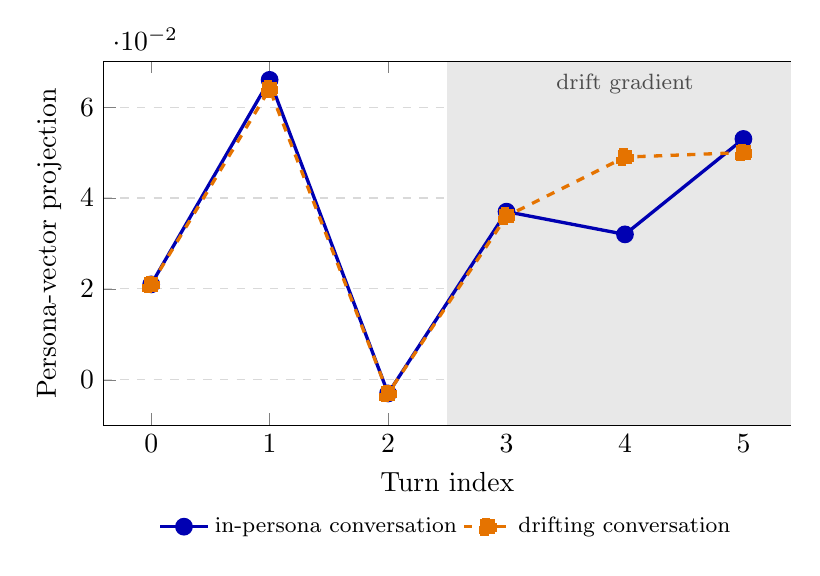
\begin{tikzpicture}
    \begin{axis}[
        width=0.85\textwidth,
        height=6.2cm,
        xlabel={Turn index},
        ylabel={Persona-vector projection},
        xmin=-0.4, xmax=5.4,
        ymin=-0.01, ymax=0.07,
        xtick={0,1,2,3,4,5},
        ymajorgrids=true,
        grid style={dashed, gray!30},
        legend style={at={(0.5,-0.22)}, anchor=north, legend columns=2, font=\footnotesize, draw=none},
        mark size=2.6pt,
      ]
      % Shaded drift gradient band (turns 3-5)
      \addplot[fill=gray!18, draw=none, forget plot] coordinates {(2.5,-0.01) (5.4,-0.01) (5.4,0.07) (2.5,0.07)} -- cycle;
      \node[font=\footnotesize, gray!60!black] at (axis cs:4, 0.065) {drift gradient};
      % In-persona trace
      \addplot[blue!70!black, mark=*, very thick] coordinates {(0,0.021) (1,0.066) (2,-0.003) (3,0.037) (4,0.032) (5,0.053)};
      % Drifting trace
      \addplot[orange!90!black, dashed, mark=square*, very thick] coordinates {(0,0.021) (1,0.064) (2,-0.003) (3,0.036) (4,0.049) (5,0.050)};
      \legend{in-persona conversation, drifting conversation}
    \end{axis}
  \end{tikzpicture}
  \caption{Per-turn drift-projection trace, Gemma-2-9B-Instruct at 4-bit, cs\_tutor persona, layer 8, generation-scope extraction. Same user turns, identical prompt prefix, only the assistant content differs between conditions. The shaded band marks the drift-gradient turns (3 through 5). The two traces are indistinguishable; absolute mean-delta over drift turns is 0.004. Source: \texttt{results/drift\_trajectory/<gemma-gen-run>/}.}
  \label{fig:drift-trajectory-cell}
\end{figure}

\subsection{Statement of the finding}
\label{sec:experiment-2-finding}

Persona vectors as published\autocite{chen2025personavectors}, validated cleanly on contrast prompts in Experiment 1 (\auroc{} 1.000 with controls intact), do not transfer to detecting persona drift in multi-turn dialogue at inference scale on the two production-scale instruct-tuned models tested (Gemma-2-9B, Llama-3.1-8B) at 4-bit quantisation, in both prompt-scope and generation-scope extraction regimes, across the layers each backbone's middle band exposes.

Two consistent geometric facts emerged in the trajectories. Same-content turns produce identical drift readings between conditions, which confirms the experimental control (the variable that matters is the assistant content, not the prompt prefix). Diverged-content turns produce different drift readings, but not in the direction that would track persona fidelity: the signal moves, it just does not track what we hoped. Absolute drift values for in-persona content are not concentrated near the in-persona centroid; multiple personas read strongly negative on their own in-persona content. The contrast-trained direction and the conversation manifold appear roughly orthogonal in these models, not aligned.

This is the project's most substantive empirical finding. It is not a refutation of the persona-vectors paper. Experiment 1 replicated cleanly under both regimes on both backbones, so the contrast-trained direction is real. It is a refutation of an architectural assumption that the same direction would also serve as an inference-time drift gate. That assumption was implicit in the v0.3 PRD design and the published methodology does not test it directly.

\subsection{Three hypotheses, all unresolved}

Three hypotheses about the cause are on the table. The first is that the contrast-prompt setup encodes role-instruction-presence rather than generation-content-fidelity: the in-persona contrast prompt says ``As [persona.role], respond to X'' and the out-of-persona prompt says ``Ignoring that you are [persona.role], respond to X'', so the direction may pick up the literal instruction string and not the construct the experimenter intends. The second is that 4-bit quantisation disrupts the direction's usefulness even though it does not disrupt the contrast-prompt separability. The third is that the prompt-instruction-versus-generation-content distinction is fundamentally geometric in these models rather than parametric, in which case no amount of probe re-training on contrast prompts would close the gap. Distinguishing the three is thesis-bridge work.

\section{Architectural cascade}

Experiment 2's refutation cascades into four decisions, recorded as \#033 through \#036 in the project's decision log.

\textbf{M2 dropped (\#035).} M2's central operation is persona-vector projection rerank, and Experiment 2 invalidates the projection signal. Unlike M3, where the gate signal is one component of a multi-piece mechanism and can be replaced, the projection rerank is M2. No signal substitution preserves the architectural claim. Spec 06 is deprecated and the M2 row is removed from the evaluation matrix.

\textbf{M3 reverts to the v0.2 design (\#034).} The drift-gated structural commitment is preserved (cheap path versus gated path, N-candidate generation, hybrid rerank). The gate signal changes from persona-vector projection to LLM-as-judge. The hybrid ranker simplifies from three signals (CharacterRM + LLM judge + persona-vector projection) to two (CharacterRM + cross-family LLM judge). Spec 07 is rewritten to v3.1.

\textbf{B3 deferred (\#036).} B3 was the activation-steering baseline: persona-vector addition to the residual stream at generation time (CAA pattern\autocite{caa2023, repe2023}). Two readings of B3 are now plausible: either the steering still has measurable effect at inference time (the Anthropic and Assistant-Axis evidence supports this) or the same gap that breaks drift detection breaks steering at the same scale. We do not have the data to distinguish them. The reframe-or-drop call is deferred pending M3 v3.1's empirical numbers on the counterfactual probes (Chapter~\ref{ch:mechanism-results}).

\textbf{A25 introduced.} A new assumption is registered: the LLM-as-judge gate must itself differentiate in-persona from drifting turns at the threshold magnitude on the existing drift-trajectory corpus, otherwise M3 v3.1 has the same problem as M3 v3 with a different scapegoat. The drift-gate calibration sweep in Section~\ref{sec:experiment-2-architecture-fixed} addresses this.

\subsection{Drift-gate calibration after the cascade}
\label{sec:experiment-2-architecture-fixed}

The four-judge cross-tier calibration sweep on the drift-trajectory corpus is the empirical follow-up to A25. Llama-3.1-8B (local), Prometheus-2-7B (local), Qwen2.5-7B (local), and GLM-4.7 (NVIDIA Build free-tier API) are run as candidate gate judges on 30 conversations with the v3 prompt template. The headline metric is the differential in flag rate between drifting and in-persona conditions; the secondary axes are the refined and sharp subsets where the drift gradient is more pronounced.

\begin{table}[H]
  \centering
  \small
  \caption{Four-judge cross-tier gate calibration on the drift-trajectory corpus. Headline $\Delta$ is the flag-rate differential between drifting and in-persona conditions. Refined $\Delta$ excludes turns hand-labelled as subtle-drift; sharp $\Delta$ uses only the full-break and clear-drift subsets.}
  \label{tab:gate-calibration}
  \begin{tabularx}{\textwidth}{l c c c c c X}
    \toprule
    \textbf{Judge (tier)}            & \textbf{Headline $\Delta$} & \textbf{Refined $\Delta$} & \textbf{Sharp $\Delta$} & \textbf{Axis populated} & \textbf{Malformed} & \textbf{Verdict} \\
    \midrule
    Llama-3.1-8B (local) + v3        & $+0.20$ & ---     & ---     & 0/30  & low  & empty axes \\
    Prometheus-2-7B (local) + v3     & $0.00$  & $0.00$  & $0.00$  & 0/30  & 30/30 & format-incompatible \\
    \textbf{Qwen2.5-7B (local) + v3} & $\mathbf{+0.40}$ & $+0.43$ & $+0.60$ & 30/30 & 1/30  & \textbf{weak (best open-model)} \\
    GLM-4.7 (API free-tier) + v3     & $+0.13$ & $+0.25$ & $+0.44$ & 30/30 & 0/30  & weak (sharp-band) \\
    \bottomrule
  \end{tabularx}
\end{table}

The operational pick is Qwen2.5-7B-Instruct on the v3 prompt template. The cross-tier ceiling is robust: going from local 7-to-9B open-model to a frontier API-tier judge did not push the headline above $+0.40$. The bottleneck is the corpus's authored content and the judge's context confusion, not judge capability. The threshold defaults to 0.5 confidence; the threshold-sensitivity sweep on the Spec-04 pilot conversations shows the gate-trigger rate flat at 50\% across thresholds in $\{0.3, 0.4, 0.5, 0.6, 0.7\}$ because Qwen's confidences cluster at exactly two values on this bench (1.00 for ok, 0.80 for drift).

M3 v3.1 ships with this configuration. The headline empirical question now is whether the v3.1 gate produces architecturally meaningful results on the counterfactual-retrieval probes, which Chapter~\ref{ch:mechanism-results} answers.
